\section{Thermal Engineering}
\f{general task}
\begin{itemize}
 \item engineering: define requirements and design
 \item analysis: establish thermal mathematical model (TMM), perform distribution calculations
 \item test: plan, perform, evaluate realistic tests
\end{itemize}

\f{satellite thermal control -- requirements}
\begin{itemize}
 \item temperature limits!
 \item temperature gradients, -stability, -uniformity
 \item heatflux, -storage
 \item power and mass-allocation
\end{itemize}

\f{heat mechanisms:}
\begin{itemize}
 \item radiation: transfer via electromagnetic waves
 \item conduction: transfer via fluids and solids in absense of fluid motion
 \item convection: transfer in a flowing fluid and between fluid and wall (mostly irrelevant in satellites)
\end{itemize}

\f{thermo optical properties of materials}
\begin{figure}[ht!]
 \centering
 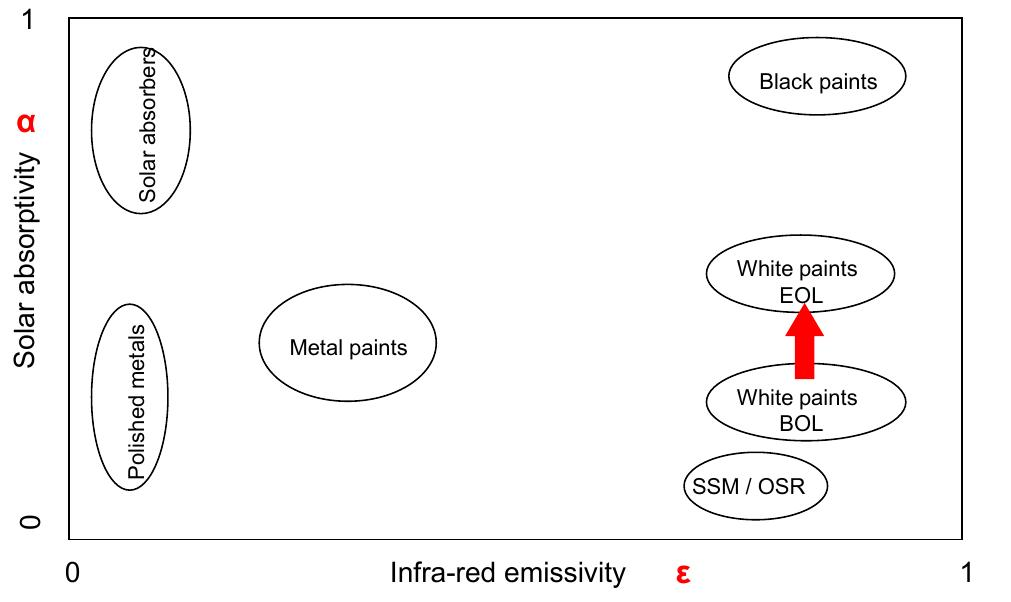
\includegraphics[scale=0.6]{thermooptical}
\end{figure}

\f{global energy balance}\\
\begin{tabular}{ll|ll}
 \tabitem Solar intensity & $\dot{q}_S = 1316\dots1428 \frac{W}{m^2}$ &  \tabitem Earth albedo & $\dot{q}_A = 0.2\dots0.4\dot{q}_S$ \\
 \tabitem Earth IR Radiation & $\dot{q}_E = 189\dots261 \frac{W}{m^2}$ &  \tabitem Absorbtivity Coefficient& $\alpha = 0\dots 1$ \\
 \tabitem Emissivity Coefficient & $\varepsilon = 0\dots 1$ &  \tabitem View Factor & $\phi = 0\dots 1$ \\
\end{tabular}

\f{orbital environment and load cases:}
\begin{itemize}
 \item external loads (sun, earth, moon...)
 \item LEO, GEO, lagrange, eclipse?
 \item orientation (earth, sun, deepspace?)
 \item operating modes
 \item mission scenario
\end{itemize}

\f{typical design load cases}\\
\begin{tabular}{l|l|l}
 & cold case & hot case \\
 \hline
 environment& cold external, BOL& hot external, EOL\\
 solar intensity& min $(\sim1320 \frac{W}{m^2})$ & max $(\sim1420 \frac{W}{m^2})$\\
 earth albedo& min $(\sim0.2)$ & max $(\sim0.4)$\\
 earth IR radiation & min $(\sim200 \frac{W}{m^2})$& max $(\sim260 \frac{W}{m^2})$\\
\end{tabular}

\f{thermal design -- approach}
\begin{itemize}
 \item insulate against environment
 \item minimize absorbed heat
 \item balance internal heat
 \item define radiator-areas and distribute heat
 \item install thermal control hardware
 \item analyze and verify TCS (thermal control system)
\end{itemize}

\f{critical components}
\begin{itemize}
 \item batteries
 \item detectors and sensors (instrument \& star)
 \item optical equipment
 \item mechanisms, tubes, propulsion systems
\end{itemize}

\f{thermal control hardware}
\begin{itemize}
 \item insulation, surface coating
 \item thermal interfillers
 \item thermal doublers, heat straps, heatpipes
 \item electrical heaters, temperature sensors
\end{itemize}





